\chapter{Exploratory Data Analysis}

\section{Descriptive Statistics}
\subsection{Geospatial Distribution}
\begin{figure}[H]
  \centering
  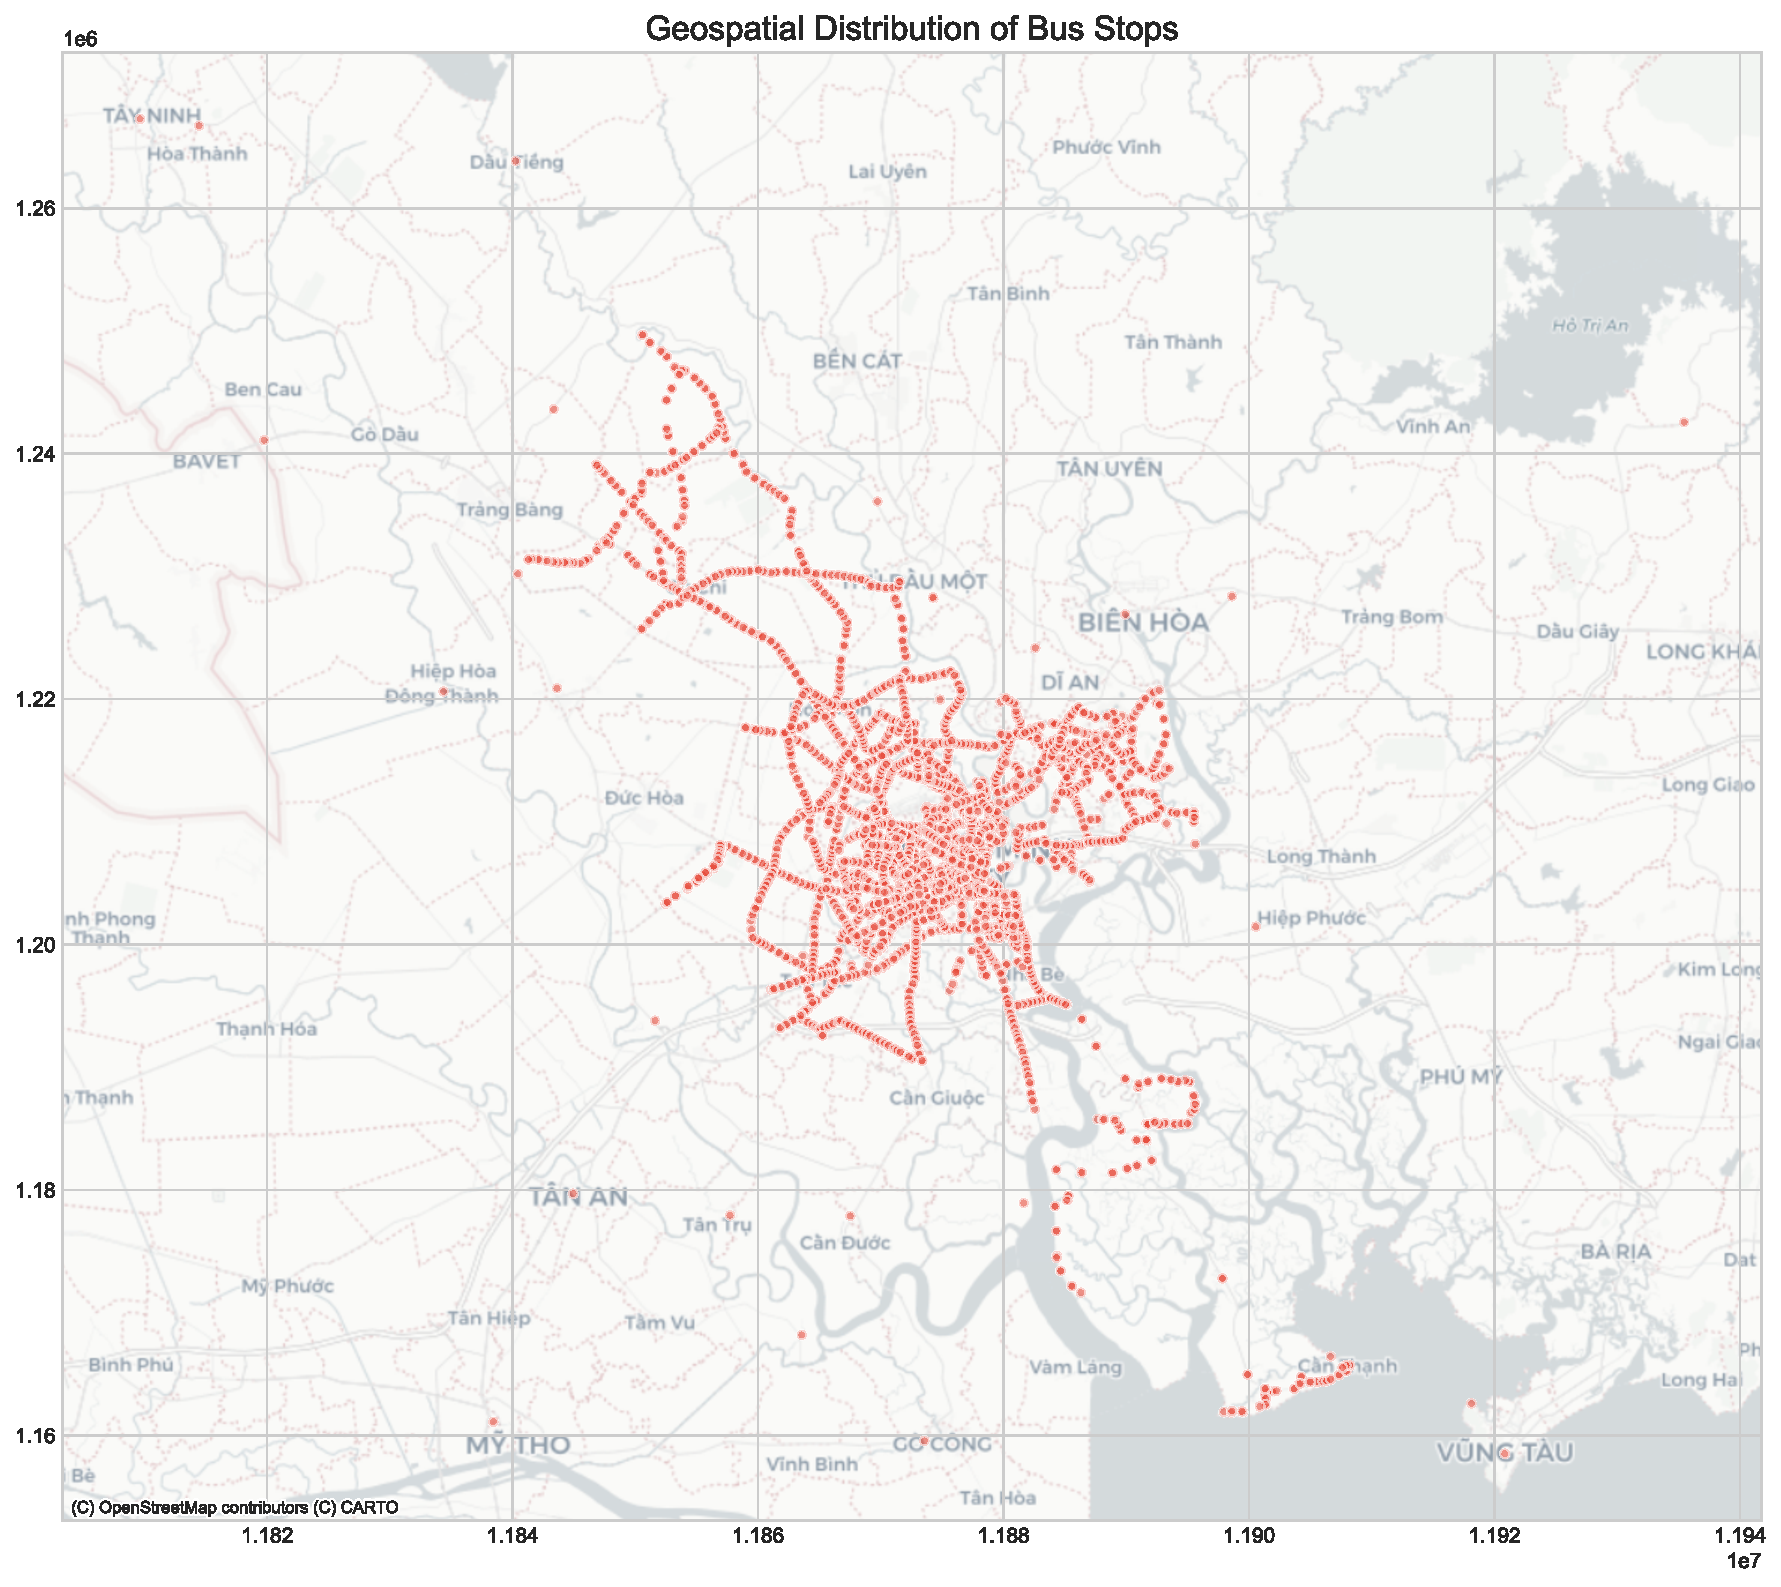
\includegraphics[width=\textwidth]{figures/bus_stops_map_with_background.pdf} 
  \caption{Geographical Distribution of Bus Stops in Ho Chi Minh City}
\end{figure}

This report provides a descriptive analysis of the Ho Chi Minh City bus network based on the provided \texttt{stops.csv} dataset and geospatial visualizations. The network consists of \textbf{4,343 unique bus stops}, serving as the primary public transport nodes for the city.

\textbf{Network Scale \& Geographic Coverage}\\
The bus network covers a wide geographic area, extending from the dense city center to suburban and rural districts.

\begin{itemize}
    \item \textbf{Total Stops:} 4,343
    \item \textbf{Geographic Center:} Latitude $10.80^\circ$N, Longitude $106.66^\circ$E (approx. Tan Binh/Phu Nhuan District).
    \item \textbf{North-South Extent:} $\sim 106$ km (From $10.35^\circ$N to $11.31^\circ$N).
    \item \textbf{East-West Extent:} $\sim 123$ km (From $106.09^\circ$E to $107.22^\circ$E).
\end{itemize}

\textbf{Location Type Analysis}\\
By analyzing common keywords in the stop names, we identified the primary types of infrastructure served by the bus network. The data indicates a strong focus on educational institutions and markets.

\begin{table}[H]
    \centering
    \caption{Distribution of Stops by Location Type}
    \vspace{0.2cm}
    \begin{tabular}{|l|l|c|}
        \hline
        \textbf{Location Type} & \textbf{Common Keywords} & \textbf{Count} \\
        \hline
        Education & \textit{Trường, Đại học, Cao đẳng} & 482 \\
        \hline
        Spiritual/Community & \textit{Chùa, Nhà thờ, Đình} & 368 \\
        \hline
        Workplaces & \textit{Công ty, Khu công nghiệp} & 300 \\
        \hline
        Commerce & \textit{Chợ, Siêu thị} & 256 \\
        \hline
        Healthcare & \textit{Bệnh viện, Trạm y tế} & 186 \\
        \hline
        Transport Hubs & \textit{Bến xe, Ga} & 119 \\
        \hline
    \end{tabular}
\end{table}

\textbf{Core Density:} Approximately 50\% of all bus stops are concentrated within a high-density urban core defined by the interquartile range:
\begin{itemize}
    \item \textbf{Latitude Range:} $10.75^\circ$N -- $10.85^\circ$N
    \item \textbf{Longitude Range:} $106.61^\circ$E -- $106.71^\circ$E
\end{itemize}
This area corresponds to the central districts (D1, D3, D5, D10, Phu Nhuan, and Binh Thanh).

\textbf{Outliers and Remote Connectivity:} The analysis identified \textbf{344 geographical outliers}. These stops represent the network's reach into remote or rural areas, such as:
\begin{itemize}
    \item \textbf{North:} Cu Chi and Tay Ninh border (e.g., stops like \textit{Tỉnh lộ 6}).
    \item \textbf{South:} Can Gio biosphere reserve (sparse connectivity).
    \item \textbf{West:} Binh Chanh and Long An border.
\end{itemize}


\textbf{Visual Structure}\\
Based on the generated map above, the network exhibits a \textbf{radial structure}:
\begin{enumerate}
    \item A dense central cluster representing the urban core.
    \item Linear extensions (``tentacles'') following major highways (e.g., Highway 22, Highway 1A) connecting the center to satellite towns.
\end{enumerate}


\subsection{Numerical Variables}
\begin{figure}[H]
  \centering
  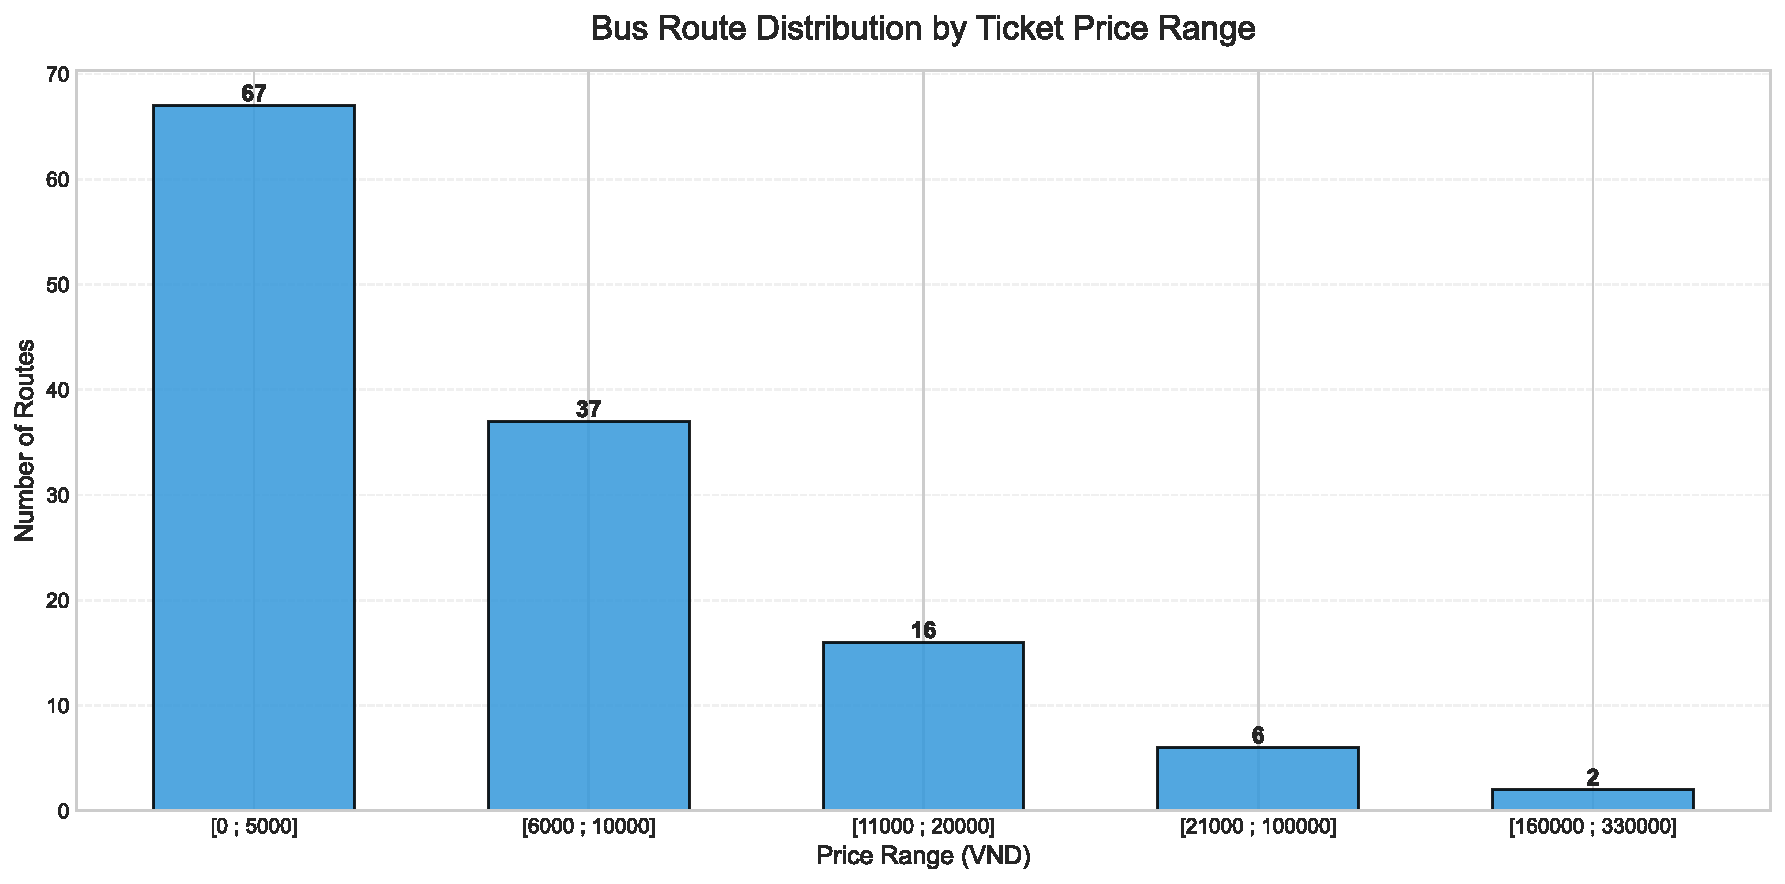
\includegraphics[width=\textwidth]{figures/bus_fee_ranges_en.pdf}
  \caption{Distribution of Ticket Fees for Bus Routes} 
\end{figure}

Ticket Fees Analysis
The majority of bus routes are affordable city commuters, but there are significant outliers representing long-distance or tourism services.
\begin{itemize}

\item Average Fee: ~12,500 VND
\item Most Common Fee (Median): 6,000 VND
\item Price Range: 5,000 VND (min) to 330,000 VND (max)
\end{itemize}
Most Expensive Routes:
\begin{itemize}
\item City Tour (Tuyến xe du lịch vòng khu vực trung tâm): 330,000 VND - This is a sightseeing hop-on hop-off service, not a standard commute.
\item Airport to Vung Tau (Sân bay TSN – Bến xe Vũng Tàu): 160,000 VND - A premium intercity link.
\item Can Gio - Vung Tau Ferry Link: 70,000 VND.
\end{itemize}

\begin{figure}[H]
  \centering
  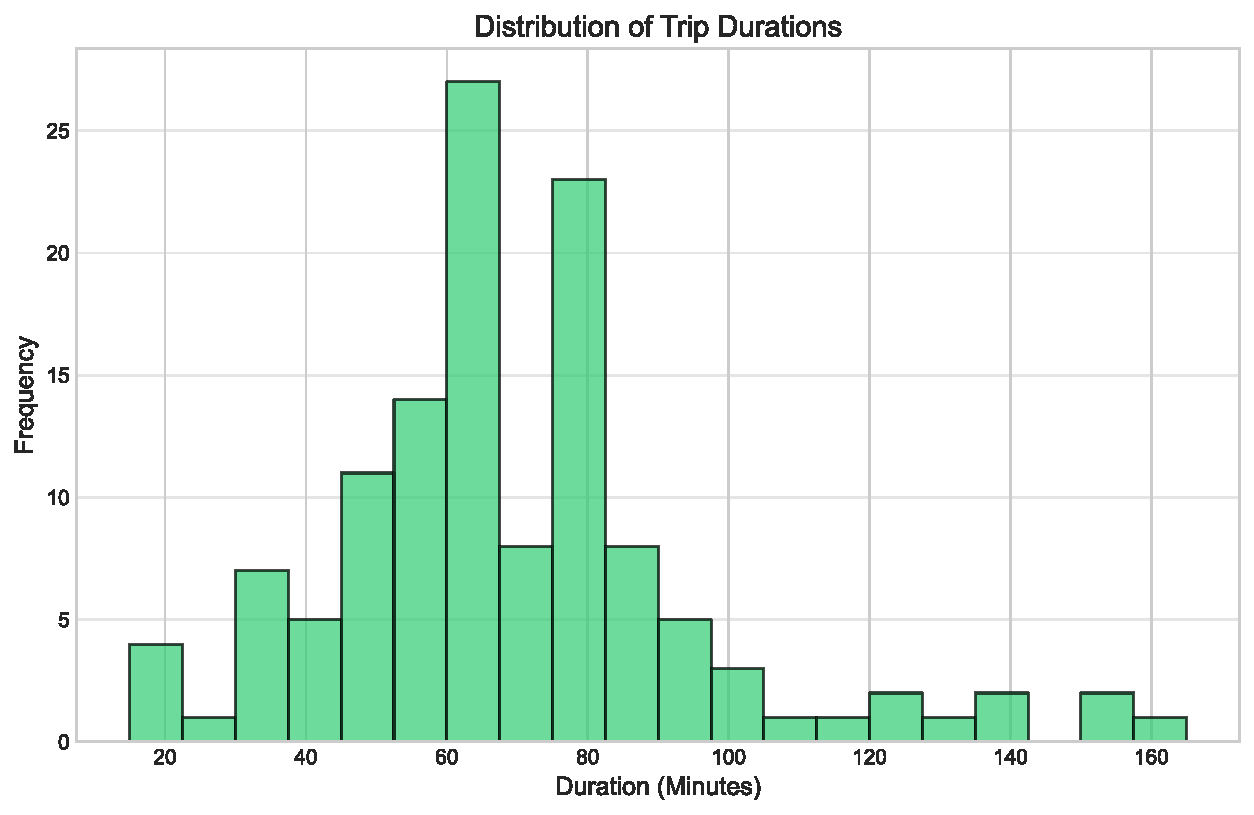
\includegraphics[width=\textwidth]{figures/trip_duration_distribution.pdf} 
  \caption{Distribution of Trip Durations for Bus Routes}
\end{figure}

Trip Duration Analysis
The busStopSpacing(time of trip) column reveals how long passengers typically spend on a bus for a full route.
\begin{itemize}
\item Average Duration: ~68 minutes
\item Standard Commute: Most trips last between 55 and 80 minutes.
\item Shortest Route: 15 minutes (likely a short shuttle or feeder service).
\item Longest Route: 165 minutes (~2.75 hours).
\end{itemize}

Based on the analysis, we build an algorithm to estimate the travel time that nearly matches the actual trip duration provided in the dataset.

\begin{itemize}
    \item Implements a modified \textbf{A*} search algorithm that considers:
    \begin{itemize}
        \item Distance between stops.
        \item Transfer penalties between routes.
        \item Starting penalty for initial waiting time.
        \item A \textbf{transfer penalty} is added when switching between routes.
    \end{itemize}

    \item The cost function is defined as:
    \[
    \text{cost} = \text{currentcost} + \frac{\text{edgeDist}}{v} + \text{transferPen} \cdot p + c \cdot \text{fare}
    \]
    \begin{itemize}
        \item \textbf{currentcost}: accumulated cost to reach the current node.
        \item \textbf{edgeDist}: distance (in meters) of the current bus segment.
        \item \textbf{transferPen}: transfer penalty, equal to the average bus spacing / waiting time; set $\text{transfer\_pen} = 0$ if there's no transfer between routes.
        \item $v$ (\text{m/s}): average bus speed, assumed to be \textbf{7 m/s}.
        \item $p$: constant coefficient that amplifies the importance of bus transfer penalties.
        \item $c$: constant coefficient that amplifies the importance of bus fare.
        \item \textbf{fare}: bus fare cost; $\text{fare} = 0$ if there's no route transfer.
    \end{itemize}
\end{itemize}

\begin{align*}
    \text{WorstCaseDuration} &= \text{TotalCost} - c \cdot \text{TotalFares} - (p-1) \cdot \text{TotalWait} + \text{walkDistance} \cdot \text{walkSpeed} \\
    \text{BestCaseDuration} &= \text{WorstCaseDuration} - \text{TotalWait}
\end{align*}

The algorithm can compare multiple potential starting stops.


\section{Analysis of Relationships}

\begin{figure}[H]
  \centering
  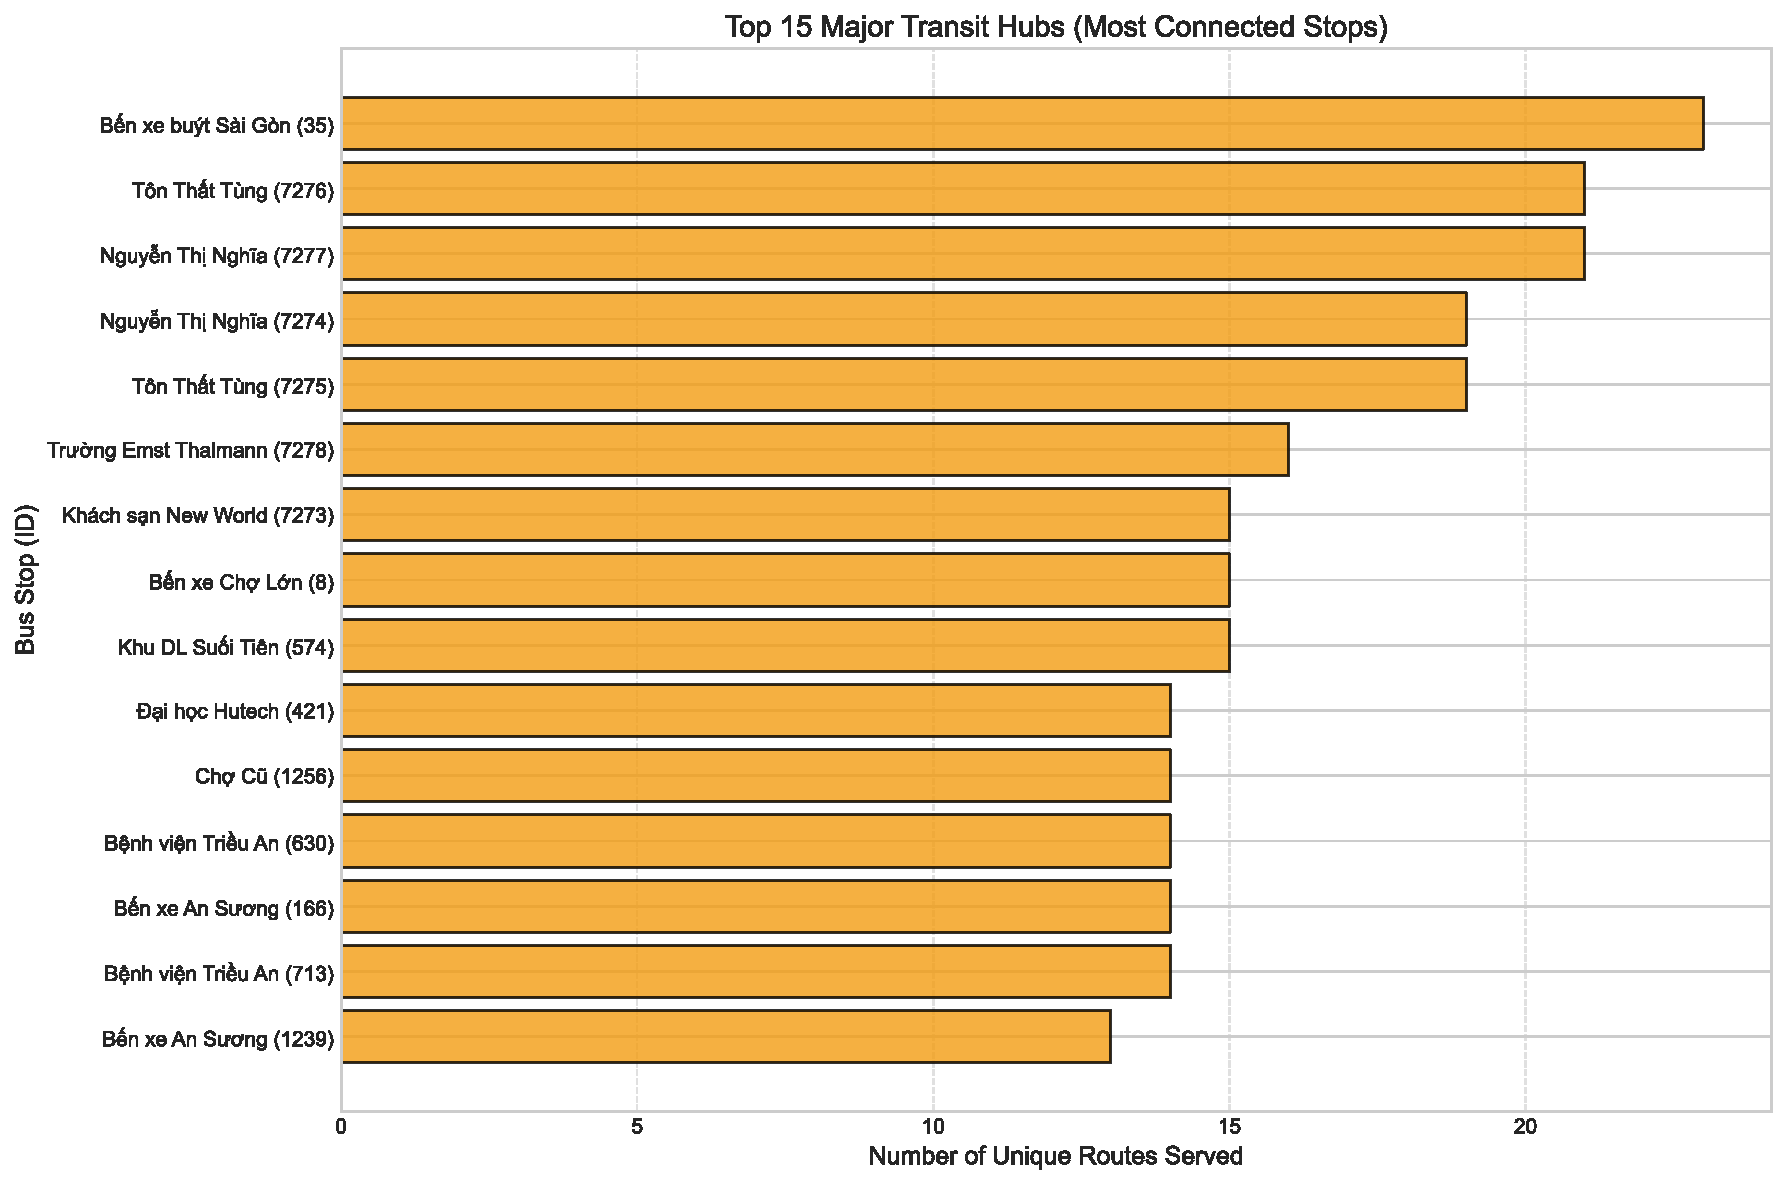
\includegraphics[width=\textwidth]{figures/transit_hubs.pdf} 
  \caption{Proximity of Bus Stops to Major Transit Hubs in Ho Chi Minh City}
\end{figure}

Based on the \texttt{trips.csv} dataset, we analyzed the physical connections (edges) that define the bus network structure.

\textbf{Network Scale}
\begin{itemize}
    \item \textbf{Nodes (Stops):} 4,343 unique locations.
    \item \textbf{Edges (Links):} 10,459 connections between stops.
    \item \textbf{Routes:} 129 distinct bus lines.
\end{itemize}

\textbf{Distance Dynamics (Edge Weights)}
\begin{itemize}
    \item \textbf{Average Hop:} The average distance between two consecutive stops is \textbf{$\sim$577 meters}.
    \item \textbf{Short Hops:} 25\% of stops are less than \textbf{269 meters} apart. This indicates a highly dense network in the city center where stops are frequently placed to facilitate easy access.
    \item \textbf{Long Hops:} The data contains extreme outliers (up to 63 km), representing express routes or intercity connections.
\end{itemize}

\textbf{Route Complexity}
\begin{itemize}
    \item \textbf{Average Route Length:} $\sim$46.8 km (Total round trip).
    \item \textbf{Variation:} Routes exhibit significant variance, ranging from short shuttle services (5.5 km) to long-haul provincial connections (146 km).
\end{itemize}

\textbf{Hub Identification}
Using stop connectivity data, we identified key transit hubs in the network:\\
\textbf{The Super-Hub (Stop ID 35)}
\begin{itemize}
    \item \textbf{Name:} Bến xe buýt Sài Gòn (Ben Thanh Bus Station).
    \item \textbf{Connectivity:} Connected to \textbf{23 unique routes}.
    \item \textbf{Role:} This node serves as the absolute center of the network. Routing algorithms should prioritize this node as a primary transfer point.
\end{itemize}

\textbf{The Central-Cluster (Stops 7276, 7277, 7274)}
\begin{itemize}
    \item \textbf{Names:} Tôn Thất Tùng, Nguyễn Thị Nghĩa.
    \item \textbf{Connectivity:} Connected to \textbf{19--21 routes}.
    \item \textbf{Insight:} Geographically adjacent to Ben Thanh Market, these stops act as overflow terminals, effectively forming a larger ``Central Transit Zone.''
\end{itemize}

\textbf{Key Regional Gateways}
\begin{itemize}
    \item \textbf{Stop 8 (Bến xe Chợ Lớn):} 15 routes -- The primary hub for the West/Chinatown area.
    \item \textbf{Stop 574 (Khu DL Suối Tiên):} 15 routes -- The gateway to the East and University Village.
    \item \textbf{Stop 166 (Bến xe An Sương):} 14 routes -- The gateway to the Northwest.
\end{itemize}

\textbf{Conclusion}
The combination of connectivity data and hub identification reveals a \textbf{Hub-and-Spoke} network architecture:
\begin{enumerate}
    \item \textbf{Core:} A massive concentration of connections at the city center (Stop ID 35 and surroundings).
    \item \textbf{Spokes:} Long routes (avg 46 km) radiate outwards to regional terminals (Cho Lon, An Suong, Suoi Tien).
    \item \textbf{Implication:} Efficient navigation across the city usually requires transferring through one of the top 15 identified hubs.
\end{enumerate}




